%\documentclass[english, a4paper]{article}
\documentclass{llncs}
\usepackage{llncsdoc}

\usepackage{float}
\usepackage[pdftex]{graphicx}
\usepackage[font={small,it}]{caption}
\usepackage[caption=false]{subfig}
\usepackage{url}
\usepackage{siunitx}
\usepackage{graphicx}
\usepackage{pbox}
\usepackage{placeins}

\newcommand{\squeezeup}{\vspace{-8.9mm}}
\setcounter{secnumdepth}{3}
\addtolength{\textfloatsep}{-3mm}
\addtolength{\belowcaptionskip}{-15pt}



\title{Data Mining -- Assignment 2}

\author{Andrew Bedard (2566978) -- Artagan Malsagov (2562231)  -- Shabaz Sultan(2566703)}

\institute{}
\begin{document}
\maketitle
\section{Introduction}
The online travel agency (OTA) Expedia posed the challenge to rank hotels by their likelihood of being booked. In such a competitive market as the one of click-through purchases, properly ranking offered hotels according to user's preferences becomes indispensable for the OTA to win the sale. This requires an algorithm that can rank the hotels associated with a user search query. The use of ranking algorithms in the industry of online travel booking is uncharted territory and the challenge provided opportunities to explore. For further information on the competition see the Kaggle platform \cite{WinNT}.

This report details our approach to tackling this problem based on the search and click-through data provided by Expedia. First, a short review of the available literature on the topic is given. Then a description of the data and the task at hand is provided. This is followed up by a review of the methods and models used by us and how they held up to the challenge. Finally, we finish off with a summary and some concluding remarks.  

\section{Related work}
Here is a sample of the approaches of some of the groups that participated in the Expedia challenge. 

Let's start with the official winner of the competition, whose approach can be found in \cite{WinNT2}. For the feature engineering missing values were said to be imputed by negative values, which we believe to mean the worst case is assumed. The rationale being customers don't like to book hotels with missing values. Numerical variables were bounded to remove outliers. Negative instances of booking and clicking were down-sampled. All original features were used, plus engineered features such as averages of numerical variables, price difference and categorical features converted to numerical ones. As a model an ensemble of Gradient Boosting Machines was used. 

The official runner-up also did a lot of feature engineering. Missing values were replaced by worst-case scenarios by the same reasoning as above. For instance the missing values of competitor descriptions where replaced by zero, which means data is not available. Furthermore, certain numerical features were normalized with respect to different indicators such as the prop\_id, srch\_id and month. New features were constructed such as the difference between the visitor's starrating and the starrating given to a certain property. This gave a total of 300 features on which the models LambdaMART, SVM Rank and linear regression were used. The final model used was LambdaMART. An import aspect of LambdaMART for this problem is that it can maximize non-smooth information retrieval function such as NDCG@k, which was used as an evalutation metric in this competition.

The paper \cite{DBLP:journals/corr/LiuXZYPLSW13} details an approach which meshes together several different ranking models: logistic regression, support vector machines, random forest, gradient boosting machine, factorization machine and LambdaMART, among others. The team identified the most import features as price\_usd, prop\_starrating and prop\_location\_score2. Data was balanced for training random forest, making it feasible to train with a large number of trees.  For missing values the first quartile calculated for the prop\_id of the missing data point was used. As their ensemble the team tried different linear combinations and sought the combination that would give a better result than a single model could.
 
\section{Data description}
Given a search query $x_{i}$ and the hotels $\{h_{1}^{i},\dots,h_{m_{i}}^{i}\}$ associated with it, where $\leq m_{i} \leq 38$(the maximum number of hotels associated with any search query is not more than $38$ and not less than $4$), a ranking algorithm has to estimate the scores  $\{s_{1}^{i},\dots,s_{m_{i}}^{i}\}$ corresponding to these hotel. The scores are assigned as:
$$
s_{j}^{i}=
\left\{
	\begin{array}{ll}
		5  & \mbox{if hotel $j$ was booked }   \\
		1 & \mbox{if hotel $j$ was clicked }  \\
		0 & \mbox{if hotel $j$ was neither clicked nor booked}
	\end{array}
\right.
$$
  
The data taken from Kaggle totals about $10$ million records spanned by $336,334$ search queries, meaning at least $4$ records correspond to one search query and at most $38$. The data is divided in half into a training and test set. Each record in the training data is represented by $54$-dimensional vector, where the two class variables booking and clicking and the variables for purchase amount and position in Expedia's ranked list are not included in the test set. Indeed, in our problem the target variables to be estimated are click\_bool and book\_boolean, based on which the scores for the ranking can be assigned. The remaining $50$ variables are roughly divided into search criteria, hotel characteristics (dynamic/static), history of the user and competitive OTA information. A variable not covered by these categories is whether the search result were presented in random order or based on the ranking algorithm employed by Expedia (in some cases hotels were presented in random order to learn about user preferences).

As an evaluation metric the average NDCG over all queries is used, with $k=38$ as the truncation level. Formally, $\displaystyle DCG_{k}=\sum_{i=1}^{k}\frac{2^{rel_i}-1}{\log_{2}(i+1)}$. Here $rel_{i}$ represent the true score of the hotel ranked in position $i$. Observe that only one score can be $5$: the hotel booked. The further down the summation it is placed the more it is discounted, decreasing the score. Likewise for the hotels that were clicked and it doesn't matter in which order the clicks are placed, as long as they are ranked below the booked hotel and above the hotels booked nor clicked. The ideal ranking then gives the maximal discounted gain, $IDCG_{k}$. Consequently, $NDCG_{k}=\frac{DCG_{k}}{IDCG_{k}}$ 

\subsection{Some challenges and observations}
Some reflections on the challenges with the data and problem are in order. First, the size of the dataset is impractical for training purposes and most software might choke on it. An appropriate technique has to be used to sample a representative subset of the data.

What's more, the data is unbalanced: at most one hotel can be booked and only a few get usually clicked, meaning it might be tempting for the algorithm to always predict not booked and not clicked. Depending on the algorithm,this situation can be remedied by down-sampling the negative instances.

The data is raw and not manually checked. So another hassle concerns missing data and outliers, which has to be dealt with when training. 

The data is furthermore divided into categorical and numerical variables. The categorical variables are for instance IDs for the search queries, hotels and websites of Expedia.  

Finally, there are multiple output variables, which can be represented in different ways, namely as either a score or classes for clicks and bookings. The fact is also that the NDCG is not a smooth function of the scores, which makes it hard to involve it in an online optimization process.            

\section{Working on the data}
\textit{price\_ usd} had many outliers, these were replaced with the first quantile value, missing values in \textit{prop\_ location\_ score2, visitor\_ hist\_ adr\_ usd, visitor\_ hist\_ starrating, prop\_ review\_ score} were replaced with the mean values of each property within their country id. Zero values in \textit{prop\_ starrating, prop\_ review\_ score, prop\_ starrating} were replaced with the third quantile values within their country id. Zero values in \textit{prop\_ log\_ historical\_ price} were replaced by first quantile values. Zero values of \textit{srch\_ length\_ of\_ stay} were replaced with mean within country id.

\[\textit{ump = exp(prop\_ log\_ historical\_ price) - price\_ usd}\]
\[\textit{price\_ diff = visitor\_ hist\_ adr\_ usd - price\_ usd}\]
\[\textit{starrating\_ diff = visitor\_ hist\_ starrating - prop\_ starrating}\]
\[\textit{per\_ fee} = \frac{\textit{price\_ usd*srch\_ room\_ count}}{\textit{srch\_ adults\_ count+srch\_ children\_ count}}\]
\[\textit{score2ma = prop\_ location\_ score2*srch\_ query\_ affinity\_ score}\]
\[\textit{total\_ fee = price\_ usd*srch\_ room\_ count}\]
\[ \textit{score1d2} = \frac{\textit{prop\_ location\_ score2} + 0.0001}{\textit{prop\_ location\_ score1} + 0.0001}\]

Mostly Andy stuff.
Feature engineering and reasoning behind it.


\section{Models and evaluation}

\subsection{Monotonic utility of the variables and SVM/GBM}
This approach was heavily inspired by the presentation of the official runner-up of the competition (see \cite{WinNT2}), where among other things RankSVM was used. This methods usually relies on linear separability, so the feature engineering we want to perform should reflect.

Let's start with an obviously important variable, the price of the hotels and take the log of it. This move accentuates the linearity between the price and the target variables, because log transform result in percentage changes and this way changes at higher levels of price are not wildly different from changes at lower levels of price. This is in line with the linear requirements of SVM. In this approach the $\log_{10}$ was taken, so as to keep the engineered variable within a workable range.

A central argument in the feature engineering of the runner-up was creating variables with monotonic utility with respect to the target variables, in particular a variable that is non-increasing with respect to clicks and bookings. So as the variable increases the number of hotels clicked/booked for that variable decreases. This property comes in handy for ranking with SVM because the larger a variable for a certain hotel, the less likely that hotel is to be booked or clicked. So when training the ranking algorithm, there is a way to separate hotels that are likely to be booked from those that are not because of variables with monotonic utility.

For instance, the variable representing the star rating of the hotels does not have this monotonic utility property, as can be seen from the figure below :
 \begin{figure}[H]
     \centering
     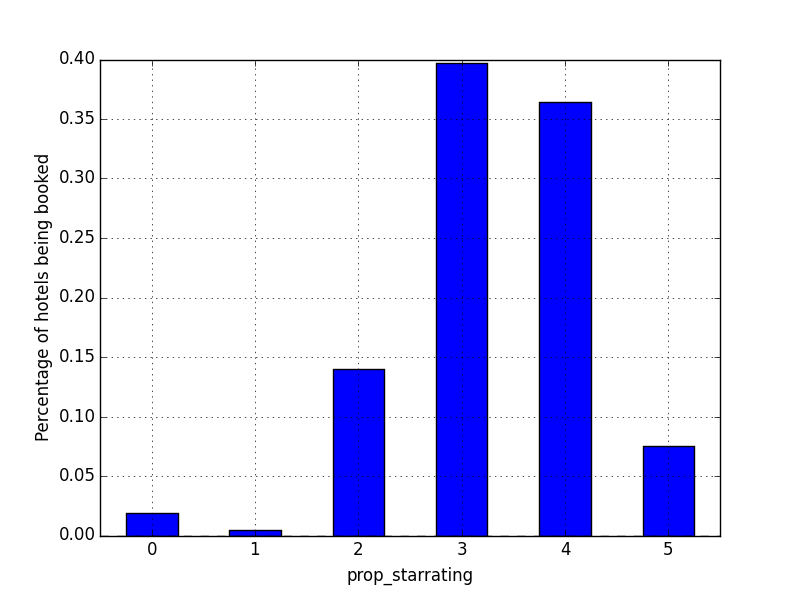
\includegraphics[width=\linewidth, height=155px]{figure_normal_starrate.png}
     \caption{Percentage of booked hotels per starrating values}
     \label{fig:prop_starrating}
 \end{figure}
\noindent However, through a simple operation a new feature can be constructed with the desired property: 
$$
\textit{prop\_starrating\_monotonic} = |\textit{prop\_starrating} -\textit{mean(prop\_starrating[booking\_bool])}|
$$
where the mean of the star-ratings of all booked hotels is subtracted from the regular variable \textit{prop\_starrating}, of which the absolute value is then taken. The intuition here is that the more a hotel star-rating deviates from the mean star-rating of the booked hotels, the less it is booked. Plotting a similar bar chart as the one above corroborates this intuition:
 \begin{figure}[H]
     \centering
     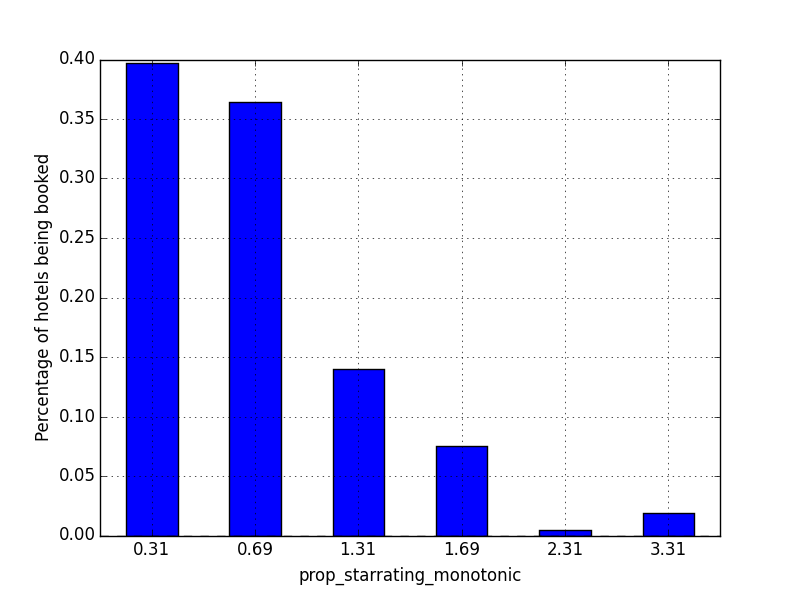
\includegraphics[width=\linewidth, height=155px]{figure_monotonic_starrate.png}
     \caption{Percentage of booked hotels per feature engineered starrating values}
     \label{fig:prop_starrating}
 \end{figure}

\subsection*{Andy}

\subsubsection*{Mr. Get'er done}


          
\bibliographystyle{plain}
\bibliography{report}
\end{document}
